%\documentclass[9pt,twocolumn]{jpc} 
%\bibliographystyle{jdc} 

%% Define some useful commands.
%\newcommand{\T}{\mathrm{T}}
%\newcommand{\tauarrow}{\stackrel{\tau}{\rightarrow}}
%\newcommand{\expect}[1]{\left< #1 \right>}

%% Set up PDF/PS automatic figure extension use.
%\newif\ifpdf \ifx\pdfoutput\undefined
%\pdffalse
%\usepackage[dvips]{graphicx}
%\DeclareGraphicsExtensions{.eps,.epsi}
%\else
%\pdfoutput=1
%\pdfcompresslevel=9
%\pdftrue
%\usepackage[pdftex]{graphicx}
%\DeclareGraphicsExtensions{.pdf}
%\fi

%% The figures are in a figures/ subdirectory.
%\graphicspath{{figures/}}

%% Import packages.
%\usepackage{times}                             	% nice fonts
%\usepackage{draftcopy}	            		% DRAFT watermark
%\usepackage{amsmath}                           	% for 'case'
%\usepackage{amsthm}                           	% for theorems and proofs
%\usepackage{mathrsfs}                          	% script math font
%\usepackage{url}                               	% allow use of URLs
%\usepackage{latexsym}                           % some math symbols, like \Box
%\usepackage{multirow}
%\usepackage{rotating}

%\setlength{\topmargin}{-1.25in}
%\setlength{\evensidemargin}{-0.25in}
%\setlength{\oddsidemargin}{-0.25in}

%\setlength{\textwidth}{17.8cm}
%\setlength{\textheight}{25.0cm}
%\setlength{\columnsep}{0.8cm}

%%\newcommand{\bfm}[1]{\mbox{\boldmath{$#1$}}}               % proper boldface for math environment
%\newcommand{\bfm}[1]{{\bf #1}}              % proper boldface for math environment

%\begin{document}

The material in this chapter was submitted to \emph{Multiscale Modeling and Simulation}, and has been accepted to appear in a Special Issue on Biological Modeling as

\flushleft{\bf Long-time protein folding dynamics from short-time molecular dynamics simulations}
\flushleft{{\bf John D. Chodera$^\dag$, William C. Swope$^\ddag$, Jed W. Pitera$^\ddag$, and Ken A. Dill$^\S$} \\
\emph{\normalsize $^\dag$ Graduate Group in Biophysics and $^\S$ Department of Pharmaceutical Chemistry, University of California at San Francisco, San Francisco, CA 94143} \\
\emph{\normalsize $^\ddag$ IBM Almaden Research Center, 650 Harry Road, San Jose, CA 95120}}

\section*{Abstract}

Protein folding involves physical timescales --- microseconds to seconds --- that are too long to be studied directly by straightforward molecular dynamics simulation, where the fundamental timestep is constrained to femtoseconds.
Here, we show how the long-time statistical dynamics of a simple solvated biomolecular system can be well-described by a discrete-state Markov chain model constructed from trajectories that are an order of magnitude shorter than the longest relaxation times of the system.
This suggests that such models, appropriately constructed from short molecular dynamics simulations, may have utility in the study of long-time conformational dynamics.

\section{Introduction}

Proteins can fold to well-defined native topologies\footnote{By \emph{native topology} or \emph{native structure}, we refer to the \emph{ensemble} of configurations sharing a coarse overall structure, or fold, with the experimental structure.} with surprising determinism.
Many small, single domain proteins can fold rapidly, reversibly, cooperatively, and without the aid of other molecular machinery.
In response to an environmental perturbation such as the introduction or removal of denaturant or a rapid change in solvent temperature, these fast-folding proteins exhibit nearly exponential relaxation kinetics with observed time constants on the order of microseconds.
Other proteins exhibit slow and complex kinetics, suggesting the presence of one or more kinetic intermediates.  
A detailed understanding of this process has been the focus of much of modern biophysics.
Ultimately, knowledge of the general mechanistic features by which proteins fold and aggregate is critical for understanding a variety of folding and misfolding diseases, elucidating principles necessary for effective protein design, and developing the basic tools needed for other related technological applications of complex molecular structures.

A description of the mechanism by which a particular protein folds must by necessity be a statistical one.  
While the initial microscopic state\footnote{By \emph{microscopic state}, we refer to the set of generalized coordinates and momenta that completely determine the microscopic state of the system, such as the phase space point.} and dynamical trajectory may differ for each molecule in an experiment, many proteins refold to their native (folded) topologies upon the restoration of native conditions with the certainty of macroscopic law \cite{anfinsen:1973a}.
A proper statistical description would summarize the salient features and relative probabilities of relevant folding routes in a way that is meaningful to the physical chemist.
This manner of model has been difficult to extract from experiments.
Despite the high time resolution possible with optical spectroscopy, the majority of these experiments rely on the observation of an \emph{ensemble} of molecules to obtain sufficient signal, resulting in the ability to observe only (possibly time-dependent) ensemble averages, rather than the behavior of any single molecule.
While observations of single molecules are now possible with fluorescence techniques, atomic force microscopy, or optical traps, high temporal resolution is sacrificed to achieve sufficient signal for reliable measurement.  
In contrast, computer simulation promises the ability to produce information with both atomic detail and high temporal resolution.

In practice, however, the presence of fast vibrational motion constrains the fundamental integration timestep to femtoseconds in order to ensure stability, limiting practical straightforward molecular dynamics simulations of atomically-detailed representations of solvated proteins to tens of nanoseconds.
As even the fastest folding proteins exhibit relaxation timescales of several microseconds \cite{kubelka:2004a}, this leads to a \emph{timescale gap} of at least two decades in time.
Using supercomputers such as Blue Gene \cite{gara:2005a} and software specialized for molecular dynamics simulations on these computer systems \cite{fitch:2003a,germain:2005a}, one can produce atomistic simulations of protein molecules with explicit representation of surrounding solvent on several microsecond timescales.
However, the number of trajectories that need be generated to provide an adequate \emph{statistical} characterization of the folding mechanism of even a single protein makes such an endeavor extremely challenging.  
Distributed computing projects like Folding@Home \cite{pande:2003a} regularly collect tens of thousands of trajectories tens of nanoseconds in length, but extracting insight about microsecond timescale dynamics from these large datasets can be difficult \cite{fersht:2002a,paci:2003a,marianayagam:2005a}.

Kinetics models may provide the necessary link between short simulations of a single molecule and long experimental observations of ensembles of molecules.  
If time evolution of a protein system is characterized by long waiting times within metastable states punctuated by infrequent transitions between these states, interstate dynamics may appear stochastic and memoryless on some short timescale.
In this case, long trajectories may be modeled as a Markov chain realized on a discrete state space of a (hopefully small) number of states.
While this model could not describe dynamical behavior at very short timescales, which is dominated by molecular motion \emph{within} a metastable state, it could nevertheless faithfully describe long-timescale transitions \emph{between} states.
This approach would have numerous advantages. 
It is precisely these slow transitions involving major structural rearrangements that are of primary interest; elimination of high-frequency detail is often desirable in aiding interpretation of trajectories.
To generate a statistical description of folding dynamics, instead of generating many simulations each long enough to contain complete folding events, we need only generate simulations long enough to characterize transition rates between pairs of conformational substates. 
Construction would therefore be amenable to parallelization on loosely-coupled grids of computer systems.  
The resulting kinetic model could then be used to compute the stochastic temporal evolution of either a single molecule or an ensemble of molecules, allowing direct comparison to data from both kinds of kinetics experiments, or to answer statistical questions about folding pathways and mechanism that are currently experimentally inaccessible.

This proposition is not entirely novel.
Several groups have constructed stochastic kinetic models from states defined by local potential energy minima of small peptides, using transition state theory to estimate interstate transition rates \cite{kunz:1995a,ball:1998b,levy:2001a,mortenson:2001a,mortenson:2002a}.
Unfortunately, the number of minima grows rapidly with increasing system size, making the procedure prohibitively expensive for larger proteins or systems containing explicit solvent molecules.
Other work \cite{degroot:2001a,swope:2004b,singhal:2004a,levy:2005a,sriraman:2005a,schultheis:2005a} has focused on the construction of discrete- or continuous-time Markovian models to describe dynamics between a small number of states.
These models, however, have yet to demonstrate that they can adequately describe the dynamics on timescales much longer than the trajectories from which the models were constructed.

Here, we present a proof of principle for how the dynamics of a solvated biomolecular system can be described using information from short simulations.
This is illustrated using terminally-blocked alanine, a system small enough that its dynamical behavior can also be thoroughly characterized by straightforward molecular dynamics simulation.  
First, a parallel tempering simulation is conducted to explore the thermally relevant regions of configuration space.
Next, a set of metastable states, corresponding to regions of configuration space with low probabilities of escape, are identified.
Due to the simplicity of the system chosen in this work, these states can readily be identified by hand.
This removes the complication of choice of state decomposition, which we shall not consider here.  
Finally, a number of short trajectories are initiated from each state (possibly in parallel) and a Markov chain model is constructed from the number of interstate transitions observed in these trajectories.

This paper is organized as follows: 
In Section \ref{long-times:section:theory}, the  Markov chain model and its method of construction are described.  
In Section \ref{long-times:section:application-to-alanine-dipeptide}, the method is applied to terminally-blocked alanine in explicit solvent.
A discussion of the significance of this result, as well as problems remaining to be solved before the method can be applied to larger biomolecules, follows in Section \ref{long-times:section:discussion}.

\section{Theory}
\label{long-times:section:theory}

\subsection{Conformational dynamics as a Markov process.}
\label{long-times:section:conformational-dynamics-as-markov-process}

Consider the dynamics of a macromolecular system in equilibrium at some temperature of interest, where we have decomposed all of configuration space into a set of $M$ disjoint states.
If we observe a trajectory of this system at times $t = 0, \tau, 2 \tau, \ldots, n \tau$, where $\tau$ denotes the observation interval, we can represent the trajectory in terms of the state the system occupies at each of these discrete times, $s_0, s_1, s_2, \ldots, s_n$.
The sequence of states produced by such a trajectory is a \emph{discrete-time stochastic process}.
If this process is a Markov chain, it must satisfy the \emph{Markov property}, whereby the probability of observing the system in state $s_n$ at the next time point, $n\tau$, given the state history $s_0, s_1,s_2,\ldots,s_{n-1}$ is independent of all but the current state $s_{n-1}$.
For a stationary process which has no explicit dependence on time, this property is given by
\begin{eqnarray}
P(s_n | s_0, s_1, s_2, \dots, s_{n-1}) &=& P(s_n | s_{n-1}) . \label{long-times:equation:markov-property}
\end{eqnarray}
As there are a finite number of states, this process can be entirely characterized by an $M \times M$ \emph{transition matrix} $\bfm{T}(\tau)$ dependent only on lag time $\tau$.
The element $T_{ji}(\tau)$ denotes the probability of observing the system in state $j$ at time $\tau$ given that it was initially in state $i$ at time $0$:
\begin{eqnarray}
T_{ji}(\tau) &\equiv& P(j | i) .
\end{eqnarray}

If we do not know the precise initial state of the system at time $0$ but only the probability the system started in each state, or if we observe an ensemble of many non-interacting systems in an experiment, we can instead consider the probability of finding one particular molecule in each state $i$ at time $n\tau$ as components of the vector of state probabilities $\bfm{p}(n\tau)$.
If the initial probability vector is given by $\bfm{p}(0)$, we can write the probability vector at some later time $n\tau$ as
\begin{eqnarray}
\bfm{p}(n \tau) \: = \: \bfm{T}(n \tau) \bfm{p}(0) \: = \: [\bfm{T}(\tau)]^n \bfm{p}(0) . \label{long-times:equation:chapman-kolmogorov}
\end{eqnarray}
This property is termed the \emph{Chapman-Kolmogorov} equation.

Once the transition matrix is known, the entire statistical dynamics of realizations of this process, corresponding to trajectories of the macromolecule under equilibrium conditions, could be extracted from it.
Macroscopically observable properties, such as the time evolution of spectroscopically observable quantities for a noninteracting ensemble of molecules, can be computed:
\begin{eqnarray}
A(n\tau) &=& \bfm{a}^\T \bfm{p}(n\tau) \nonumber \\
&=& \bfm{a}^\T [\bfm{T}(\tau)]^n \bfm{p}(0)
\end{eqnarray}
where $\bfm{a}$ denotes the vector containing the phase averages of the observable $A$ over each state.
In addition, microscopic quantities such as state lifetimes \cite{swope:2004a}, mean first-passage times \cite{singhal:2004a}, hidden intermediates \cite{ozkan:2002a}, and $P_\mathrm{fold}$ values (transmission coefficients) \cite{lenz:2004a} can be obtained.

\subsection{Construction of the Markov chain model from simulation.}
\label{long-times:section:construction-of-markov-model-theory}

For a system in which the dynamics are Newtonian but the initial configurations come from a canonical distribution, Swope et al. \cite{swope:2004a} show that the transition probability $T_{ji}(\tau)$ can be written as
\begin{eqnarray}
T_{ji}(\tau) &\equiv& \frac{\expect{\chi_j(\bfm{z}(\tau)) \chi_i(\bfm{z}(0))}}{\expect{\chi_i({\bfm{z}(0)})}} \nonumber \\
&=& \frac{\int d\bfm{z}(0) \, e^{-\beta H(\bfm{z}(0))} \, \chi_j(\bfm{z}(\tau)) \, \chi_i(\bfm{z}(0))}{\int d\bfm{z}(0) \, e^{-\beta H(\bfm{z}(0))} \, \chi_i(\bfm{z}(0))} \nonumber \\
&=& \int d\bfm{z}(0) \, p_i(\bfm{z}(0)) \, \chi_j(\bfm{z}(\tau))  
\end{eqnarray}
where $\bfm{z}$ denotes a point in phase space, $\chi_i(\bfm{z})$ denotes the indicator function for state $i$, $\beta = (k_B T)^{-1}$ is the inverse temperature, $H(\bfm{z})$ is the Hamiltonian, and $p_i(\bfm{z})$ denotes the canonical distribution restricted to state $i$:
\begin{eqnarray}
p_i(\bfm{z}) &=& \frac{e^{-\beta H(\bfm{z})} \, \chi_i(\bfm{z})}{\int d\bfm{z} \, e^{-\beta H(\bfm{z})} \, \chi_i(\bfm{z})} .
\end{eqnarray}
This result simply states the obvious: the transition matrix element $T_{ji}(\tau)$ can be estimated in a straightforward (though potentially inefficient) manner by initiating a number of simulations from configurations selected from a canonical distribution within state $i$, evolving the dynamics for a time $\tau$, and determining the fraction of trajectories that terminate in state $j$:
\begin{eqnarray}
T_{ji}(\tau) &\approx& \frac{N_{ji}(\tau)}{\sum\limits_{j'=1}^M N_{j'i}(\tau)} . \label{long-times:equation:transition-element-estimator}
\end{eqnarray}
Here, $N_{ji}(\tau)$ denotes the number of trajectories initiated from state $i$ that terminate in state $j$ at time $\tau$.  This procedure corresponds to the method proposed earlier by Swope et al. in the special case that the \emph{selection cells} from which sets of simulations are initiated are coincident with the states \cite{swope:2004a}.

We do not expect dynamics of a macromolecule in solution to resemble a Markov process for all observation intervals $\tau$, as ballistic motion dominates on very short times and sufficient time must be allowed for collisions with the solvent and decorrelation of the trajectory within a metastable state.
Imperfect definitions of the metastable states may also lead to non-Markovian behavior on short times \cite{swope:2004a}.
At sufficiently long intervals $\tau$, however, we may see that dynamics resembles a Markov process.
While it is impractical to test the condition of complete history independence (Eq. \ref{long-times:equation:markov-property}), we can simply check the (weaker) condition imposed by the Chapman-Kolmogorov equation: For transition matrices constructed for a given $\tau$, we check whether Eq. \ref{long-times:equation:chapman-kolmogorov} holds for several lag times $n = 2, 3, 4, \ldots$ to within statistical uncertainty.  If so, the Markovian model can be assumed to be a reasonable model of dynamics.

\section{Application to terminally-blocked alanine peptide}
\label{long-times:section:application-to-alanine-dipeptide}

\begin{figure}[tb]
  \begin{center}
    \resizebox{3.375in}{!}{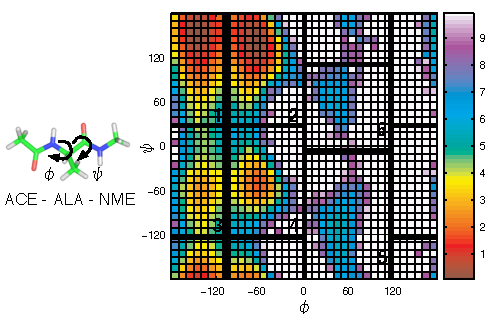
\includegraphics{chapters/mastereqn-alanine-long-times/figures/2d-pmf.pdf}}
  \end{center}
  \caption{{\bf Potential of mean force and state boundaries.}  Left: The terminally-blocked alanine peptide with $(\phi,\psi)$ torsions labeled.  Right: The potential of mean force in the $(\phi,\psi)$ torsions at 302 K estimated from the parallel tempering simulation, truncated at $10 k_B T$ (white regions), with reference scale (far right) labeled in units of $k_B T$.  Boundaries defining the six manually-identified states are superimposed and the states labeled.}
  \label{long-times:figure:2d-pmf}
\end{figure}

\begin{table}[tb]
\caption{{\bf State definitions for the manual decomposition of $(\phi,\psi)$-space into metastable states and populations at 302 K.}}
\label{long-times:table:state-definitions}
\begin{center}
\begin{tabular}{ccccc}
\hline 
      &                        & \multicolumn{2}{c}{state definitions} & \\
\cline{3-4}
state & label$^a$ & $\phi$ & $\psi$ & $P_{eq}$$^b$ \\
\hline
1 & $\mathrm{C}_5$             & $[117, \, -105)$ & $[28, \, -124)$ & .4787 (.0613) \\
2 & $\mathrm{P}_\mathrm{II}$   & $[-105, \, 0)$   & $[28, \, -124)$ & .4159 (.0486) \\
3 & $\alpha_\mathrm{P}$        & $[117, \, -105)$ & $[-124, \, 28)$ & .0425 (.0038) \\
4 & $\alpha_\mathrm{R}$        & $[-105, \, 0)$   & $[-124, \, 28)$ & .0588 (.0079) \\
5 & $\mathrm{C}_7^\mathrm{ax}$ & $[0, \, 117)$    & $[111, \, -5)$  & .0030 (.0015) \\
6 & $\alpha_\mathrm{L}$        & $[0, \, 117)$    & $[-5, \, 111)$  & .0011 (.0004) \\
\hline 
\end{tabular}
\end{center}
\footnotesize
$^a$ Corresponding state labels from \cite{roterman:1989a}.  $^b$ Equilibrium probabilities at 302 K estimated from the replica exchange simulation by WHAM, with corresponding uncertainties representing one standard deviation shown in parenthesis.
\end{table}

\subsection{System setup and equilibration.}
\label{long-times:section:system-setup-and-equilibration}

Using the {\tt LEaP} program from the AMBER7 molecular mechanics package \cite{AMBER7}, a terminally-blocked alanine peptide (sequence ACE-ALA-NME, see Figure \ref{long-times:figure:2d-pmf}) was generated in the extended conformation, with peptide force field parameters taken from the AMBER {\tt parm96} parameter set \cite{AMBER-parm96}.
The system was subsequently solvated with 431 TIP3P water molecules \cite{jorgensen:1983a} in a truncated octahedral simulation box with dimensions chosen to ensure all box boundaries were at least $7$ \AA\ from any atom of the extended peptide.
All minimization and molecular dynamics simulations were conducted using the {\tt sander} program from the AMBER7 package.
Default nonbonded cutoffs were used, bonds to hydrogen were constrained with SHAKE using a tolerance of $10^{-8}$ \cite{SHAKE}, and long-range electrostatics were treated by the particle-mesh Ewald (PME) method \cite{darden:1993a} with the default settings.

The system was first subjected to 50 steps of steepest descent energy minimization, followed by 1000 steps of conjugate gradient optimization.
To equilibrate the explicit solvent system to the appropriate volume, a 100 ps molecular dynamics simulation was performed with the temperature adjusted to 300 K and the pressure to 1 atm by the Berendsen weak-coupling algorithm \cite{berendsen:1984a} with temperature and pressure relaxation time constants of 1 ps and 0.2 ps, respectively.
The simulation box was fixed at the final size obtained from this equilibration step, with a volume of 13 232 \AA$^3$, in all subsequent simulations.

\subsection{Parallel tempering.}
\label{long-times:section:parallel-tempering}

In order to broadly explore the configuration space of the peptide and ensure that all important conformational substates were located, a parallel tempering (or replica-exchange among temperatures) molecular dynamics simulation \cite{sugita:1999a} was conducted using a parallel {\tt Perl} wrapper for the {\tt sander} program\footnote{A copy of this Perl wrapper to perform replica-exchange simulations using AMBER7 and AMBER8 can be obtained from \url{http://www.dillgroup.ucsf.edu/~jchodera/code/rex}.}.
Forty replicas were used, with replica temperatures exponentially distributed over the range 273--600 K, yielding an average exchange acceptance probability of about 50\%.
All momenta were reassigned from the Maxwell-Boltzmann distribution at the appropriate replica temperature after each exchange attempt, and constant-energy, constant-volume molecular dynamics with a 2 fs timestep was performed between exchange attempts.
The algorithm used to select pairs of replicas for temperature exchange attempts starts from the highest-temperature replica and attempts to swap the configuration for the next-lowest temperature replica using the Metropolis-like criteria, and proceeds down the temperatures in this manner.  On the next iteration, swapping attempts start from the lowest temperature and proceed upward, and this alternation in direction is continued in subsequent pairs of iterations.

Starting all replicas from the volume-equilibrated configuration described above, 100 iterations were conducted with 1 ps between exchange attempts to equilibrate the replicas to their respective temperatures.
This equilibration run was followed by a production run of 500 iterations with 20 ps between exchange attempts, a total of 10 ns/replica.
Solute configurations and potential energies from the production run  were written to disk every 0.1 ps, while full-system restart files were recorded every 1 ps for the purpose of starting new simulations from these configurations, as described in Section \ref{long-times:section:construction-from-short-trajectories}.

\subsection{State decomposition.}
\label{long-times:section:state-decomposition}

The slow degrees of freedom for terminally-blocked alanine peptide (neglecting those involving solvent motion) can be captured by the two backbone torsion angles labeled $\phi$ and $\psi$ (see Figure \ref{long-times:figure:2d-pmf}) \cite{bolhuis:2000a,ma:2005a}. To this end, the potential of mean force at 302 K was computed from the parallel tempering data using the weighted histogram analysis method (WHAM) \cite{kumar:1992a,chodera:jctc:2006} and is shown in Figure \ref{long-times:figure:2d-pmf}.  Six free energy basins are readily visible, and rectangular regions around these basins were chosen for the decomposition of all of configuration space into a set of six states.  State definitions are listed in Table \ref{long-times:table:state-definitions} and plotted as thick dividing lines in Figure \ref{long-times:figure:2d-pmf}.

\subsection{Construction of Markov chain model from short trajectories.}
\label{long-times:section:construction-from-short-trajectories}

%In order to construct a discrete-state master equation for a system exhibiting dynamics with timescales that are very long compared to timescales typically accessible my molecular dynamics simulation (such as protein folding), it is necessary to be able to be able to capture these long timescales with shorter simulations or through other importance sampling techniques for computing state-to-state transition probabilities or rates.  

%A set of 1000 NVE trajectories of 100 ps in length were initiated from each state, for an aggregate simulation time of 600 ns.  To ensure a sufficient set of starting configurations in the states of high free energy, the initial configurations were selected from the entire pool of conformations generated from the production replica-exchange simulation and selected with each snapshot selected with a likelihood appropriate to its probability of being sampled at 302 K as computed by WHAM.  Initial velocities were randomly assigned from the Maxwell distribution at the same temperature.  Figure \ref{long-times:figure:shoot-100ps:occupancy} shows the fractional occupancy of each state as a function of time for each of the six sets of initial starting states.

To construct a Markov chain model of dynamics once the states were identified, the interstate transition probabilities were computed using the procedure described in Section \ref{long-times:section:construction-of-markov-model-theory}.
A set of 1000 energy-conserving trajectories 10 ps in length were generated from a canonical distribution of initial conditions within each state.
This initial distribution was generated by selecting initial configurations from all replicas of the replica exchange simulation with a probability proportional to their weight in the canonical ensemble at 302K, as determined by WHAM, and assigning initial momenta from the Maxwell-Boltzmann distribution.
For each lag time $\tau$, the state populations, which correspond to an estimate of the transition probability $T_{ji}(\tau)$, were then obtained from Eq. \ref{long-times:equation:transition-element-estimator}.
A bootstrap procedure \cite{efron:1979a}, in which 200 replicates of 1000 trajectories from each state were chosen with replacement from the set of trajectories emanating from each state, was used to estimate the uncertainty in the observed transition probabilities.

The observed transition probabilities out of each state as a function of $\tau$ are shown in Figure \ref{long-times:figure:time-evolution-10ps}, along with the corresponding equilibrium probabilities of each state determined from the replica-exchange simulation.
None of the state populations reach their equilibrium values within 10 ps, indicating the slowest relaxation timescales are much longer, perhaps substantially so for trajectories originating from states 5 and 6.
Transition matrices at several lag times --- 0.1 ps, 1 ps, 6 ps, and 10 ps --- are shown in Table \ref{long-times:table:transition-matrices}.

\begin{figure}[tb]
  \begin{center}
    \resizebox{3.375in}{!}{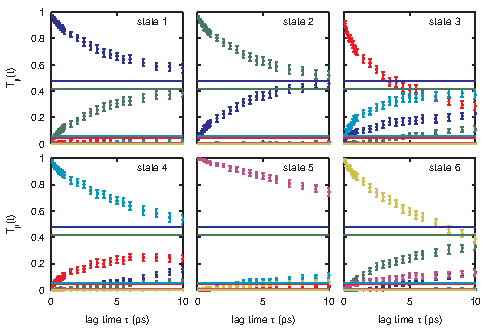
\includegraphics{chapters/mastereqn-alanine-long-times/figures/time-evolution-10ps.pdf}}
  \end{center}
  \caption{{\bf Transition matrix elements as a function of lag time estimated from 10 ps shooting trajectories.}  Each plot, labeled above by the state from which the trajectories originated, shows state-to-state transition probabilities as a function of the lag time $\tau$ estimated from a set of 1000 trajectories 10 ps in length originating from an equilibrium distribution within each state.  
   Vertical bars depict 95\% confidence intervals. 
   Equilibrium state probabilities obtained from the parallel tempering simulations are shown as solid horizontal lines in the corresponding color.}
  \label{long-times:figure:time-evolution-10ps}
\end{figure}	

\begin{table}[tbh]
\caption{{\bf Transition matrices$^a$ at several lag times estimated from set of 10 ps trajectories.}}
\label{long-times:table:transition-matrices}
\begin{center}
\small
\begin{tabular}{lcc}
\hline
$\bfm{T}(0.1~\mathrm{ps})$ & $=$ & 
$\left[
\begin{tabular}{cccccc}
.967 & .041 & .029 &      &      & .002 \\
.030 & .959 &      & .003 &      & .001 \\
.003 &      & .912 & .022 &      &      \\
     &      & .059 & .975 &      &      \\
     &      &      &      & .993 & .015 \\
     &      &      &      & .007 & .982 \\
 \end{tabular}
 \right]$ \\
\\
$\bfm{T}(1~\mathrm{ps})$ & $=$ & 
$\left[
\begin{tabular}{cccccc}
.856 & .161 & .096 & .011 & .002 & .004 \\
.130 & .835 & .008 & .007 &      & .086 \\
.014 & .002 & .701 & .109 & .001 &      \\
     & .002 & .195 & .873 & .014 &      \\
     &      &      &      & .966 & .047 \\
     &      &      &      & .017 & .863 \\
 \end{tabular}
 \right]$ \\
\\
$\bfm{T}(6~\mathrm{ps})$ & $=$ & 
$\left[
\begin{tabular}{cccccc}
.642 & .400 & .190 & .068 & .010 & .069 \\
.324 & .586 & .069 & .043 & .011 & .268 \\
.023 & .009 & .373 & .251 & .017 & .002 \\
.011 & .005 & .367 & .637 & .075 & .004 \\
     &      & .001 & .001 & .839 & .104 \\
     &      &      &      & .048 & .553 \\
 \end{tabular}
 \right]$ \\
 \\
$\bfm{T}(10~\mathrm{ps})$ & $=$ & 
$\left[
\begin{tabular}{cccccc}
.573 & .459 & .232 & .157 & .022 & .138 \\
.385 & .520 & .110 & .072 & .033 & .333 \\
.018 & .013 & .286 & .235 & .030 & .005 \\
.022 & .008 & .371 & .535 & .111 & .009 \\
     &      & .001 & .001 & .745 & .127 \\
.002 &      &      &      & .059 & .388 \\
 \end{tabular}
 \right]$ \\
 \hline
 \end{tabular}
\end{center}
\footnotesize
$^a$ Blank entries denote estimated transition probabilities of zero.
\end{table}

\subsection{Comparison with long trajectories.}

To determine the accuracy with which transition matrices constructed from different lag times from short (10 ps) simulations are able to reproduce the statistical dynamics over long times (approximately 100 ps), state populations for an ensemble of trajectories emanating from each state were computed from the model and compared to the observed time evolution of a separate set of long trajectories.
For this comparison, 1000 trajectories 100 ps in length were initiated from each state, using the same protocol in Section \ref{long-times:section:construction-from-short-trajectories}.
Figure \ref{long-times:figure:time-evolution-with-model} shows the time evolution of state populations from these trajectories (along with corresponding uncertainties) as a function of time. 
Superimposed are state populations computed by Eq. \ref{long-times:equation:chapman-kolmogorov} from the transition matrices constructed for different lag times $\tau$ from the short simulations described in Section \ref{long-times:section:construction-from-short-trajectories}.
These are connected by straight line segments solely to guide the eye; the model cannot make predictions for the populations at times that are not integral multiples of the lag time $\tau$.

The transition probabilities are poorly reproduced in the model constructed with a lag time of only 0.1 ps.
Apparently, this time is so short that the system does not behave in a Markovian manner on this timescale.
At a lag time of 1 ps, the agreement between the model and long simulations is clearly better, though there are still visible systematic deviations.
By a lag time of 6 ps, the agreement is excellent.
The model constructed from a lag time of 10 ps also shows excellent agreement, but by this time, the temporal resolution has started to become rather poor.
Information about the system is only known for times that are integral multiples of 10 ps.
One can imagine that the most useful model would be constructed from the shortest lag time at which dynamics is Markovian, as this model has the highest temporal resolution while still correctly describing long-time dynamics

\begin{figure*}[tbp]
 \begin{center}
    \resizebox{\textwidth}{!}{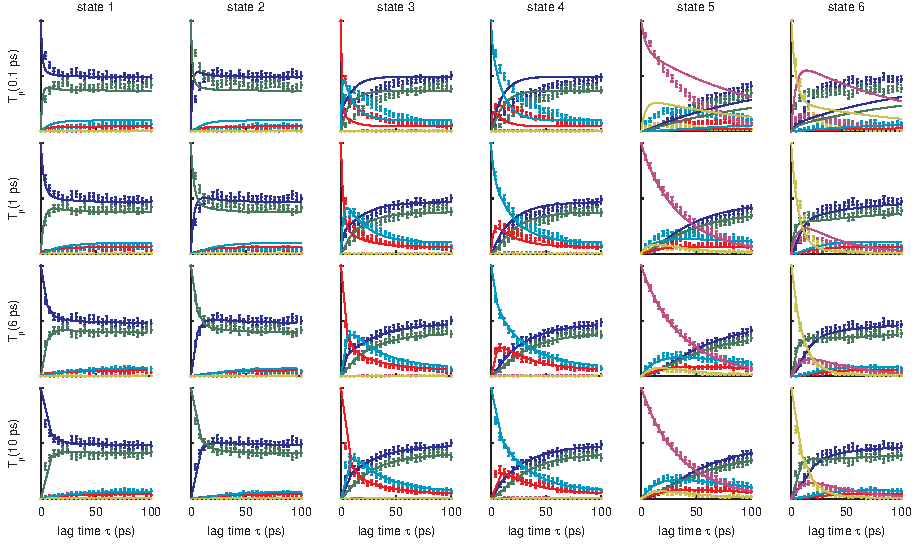
\includegraphics{chapters/mastereqn-alanine-long-times/figures/time-evolution-with-model.pdf}}
  \end{center}
  \caption{{\bf Temporal evolution of state populations from Markov chains constructed at different lag times compared with long simulations.}  Evolution of state probabilities from an ensemble prepared at equilibrium within each state for Markov model estimated from the set of 10 ps shooting trajectories (solid lines) superimposed on fractional population of each state as a function of time for ensemble of 100 ps trajectories initiated from each state (points).  
Vertical bars depict 95\% confidence intervals in state populations estimated from the long trajectories.}
  \label{long-times:figure:time-evolution-with-model}
\end{figure*}

\subsection{Long-time dynamics from the Markov chain model.}

As an illustration of the utility of the Markov chain model, Figure \ref{long-times:figure:artificial-trajectory} depicts an \emph{artificial} trajectory generated by realization of the Markov process, 10 ns in length, three orders of magnitude longer than the short trajectories used to construct the model.
While statistical properties of the dynamics can also be extracted in other ways, such as through an eigenvalue decomposition, it may be useful to generate artificial trajectories and analyze them directly.
Note the infrequent sampling of states 5 and 6, states with very small equilibrium probabilities, and the long dwell times in the region formed by stable states 1 and 2.

\begin{figure*}[tbp]
 \begin{center}
    \resizebox{\textwidth}{!}{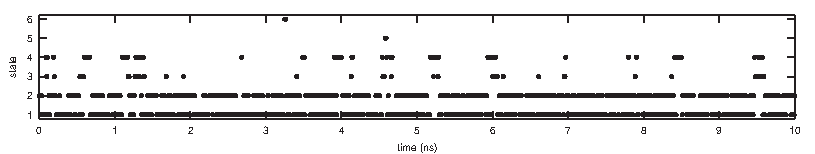
\includegraphics{chapters/mastereqn-alanine-long-times/figures/artificial-trajectory.pdf}}
  \end{center}
  \caption{{\bf An artificial trajectory generated from the transition matrix constructed from a lag time of 10 ps.}}
  \label{long-times:figure:artificial-trajectory}
\end{figure*}
  
\section{Discussion}
\label{long-times:section:discussion}

We have demonstrated that a Markov model constructed from simulations roughly one order of magnitude shorter than the slowest relaxation time in the system is sufficient to capture the long-time dynamics of a simple biomolecular system, terminally-blocked alanine peptide in explicit solvent.
Instead of generating large numbers of long trajectories to statistically characterize dynamics, we require only a sufficient number of trajectories to estimate transition probabilities between pairs of states.
In addition, these trajectories need only be long enough for interstate dynamics to appear Markovian.
Once so constructed, the model can be used to answer various questions of interest regarding the long-time statistical dynamics without the need to perform additional simulations.

While it is impossible to predict what the minimum trajectory length required for Markovian behavior will be for other, larger systems, it is important to recall that most proteins fold on the millisecond to second timescale.
Even fast folding proteins can require tens of microseconds to fold \cite{kubelka:2004a}.
To bring the treatment of these systems within the realm of feasibility, the Markov time would need to remain sufficiently short to allow the collection of a significant number of trajectories despite the presence of relaxation times many orders of magnitude longer.
No statement can yet be made about the number of states necessary to model more complex systems, or whether this number might make this approach prohibitively expensive.

To determine the lag time to construct the transition matrix so that the Markov chain is an accurate description of long-time dynamics, it was necessary to compare to an additional set of long trajectories.
This, of course, defeats the utility of a model constructed from short trajectories.
The question of how best to validate a Markov chain model constructed from short trajectories without additional long-time information is a topic of active research.
In the worst case, the transition matrix constructed from a lag time of 0.1 ps clearly disagree at long times --- this disagreement is clearly an indicator of disagreement at long times.
Other methods, such as tests of eigenvalue behavior \cite{swope:2004a} or direct tests of Markovity \cite{park:2006a}, may provide alternatives.

In this work, we have avoided the issue of how best to define the number and location of states used for construction of the Markov model.
Ideally, these states will be significantly \emph{metastable} so that the system rapidly loses memory of its previous location after entering a state, before making a transition to another state.
For the system considered, the slow degrees of freedom were known beforehand, so the potential of mean force in these coordinates revealed a useful set of states.
In more complex systems, the coordinates in which dynamics is slow will be much more difficult to discern; some automatic method for the identification of metastable states is necessary, which is the subject of work soon to be reported \cite{singhal:2006a}.

Here, we employed the most straightforward approach to estimating interstate transition probabilities, whereby a large number of short trajectories are initiated from equilibrium within each state.
While this approach is amenable to distributed or grid computing, the metastable nature of well-chosen states will result in many of these trajectories simply remaining in their state of origin, rather than contributing to estimates of the off-diagonal elements of the transition matrix.
It is precisely these off-diagonal elements that are critical in determining which trajectories through state space are most likely.
Algorithms employing importance sampling techniques in \emph{trajectory} space --- such as transition path sampling \cite{dellago:1998a}, transition interface sampling \cite{vanerp:2003a}, and the string method \cite{e:2002a} --- may provide an efficient way to compute these interstate transition probabilities.

\section{Acknowledgements}

JDC was supported by Howard Hughes Medical Institute and IBM predoctoral fellowships.
WCS acknowledges support from NSF MRSEC Center on Polymer Interfaces and Macromolecular Assemblies DMR -- 0213618, and KAD the support of NIH grant GM34993.
JDC gratefully acknowledges Libusha Kelly (UCSF) for critical reading of this manuscript and Nina Singhal (Stanford) for stimulating discussion and insightful criticism.

%\bibliography{mastereqn-alanine-long-times}

%\end{document}
